\chapter{АНАЛИЗ ПРЕДМЕТНОЙ ОБЛАСТИ СИСТЕМЫ УПРАВЛЕНИЯ ШАГАЮЩИМИ РОБОТАМИ}
В этой главе приводится обзор существующих на данных момент видов роботов, которые имеют непосредственное отношение к данной работе. Рассматриваются как шагающие роботы в целом, так и инсектоморфные, являющихся подвидом шагающих. В конце главы также рассматриваются методы управления такими роботами.

\section{Шагающие роботы}

Шагающие роботы являются важной альтернативой роботам, использующим колесные и гусеничные движители, поскольку большая часть земной площади редко представляет из себя даже грунтовую дорогу. Таким образом, если ездящие роботы более специализированы и лучше приспособлены для плоских поверхностей - они могут двигаться быстрее и лучше ориентироваться в пространстве, используя различные системы навигации, то шагающие роботы могут использоваться в более разнообразных условиях. Такие роботы следуя природе, имеют возможность перемещаться по пересеченной местности или даже подниматься по лестнице или преодолевать препятствия в стандартной бытовой ситуации, на что не способно большинство ездящих роботов. Также ноги шагающего робота наносят значительно меньший ущерб местности, чем колесные или гусеничные машины. Кроме того, положение тела робота может быть изменено, при удержании ног на земле, таким образом, добавляется еще одна степень свободы для выполнения различных задач. Пример перемещения робота по пересеченной поверхности приведен на рисунке \ref{img:motion_planning} на котором отражен принцип работы модуля motion planner, отвечающего за вычисление последовательности действий, необходимых для перемещения ног от исходной точки к конечной, с учетом рельефа поверхности.

\begin{figure}
	\centering
	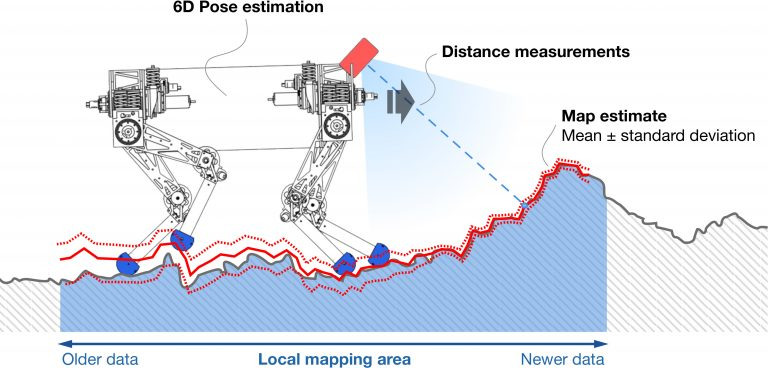
\includegraphics[]{img/robot_walks}
	\caption{Работа motion planner на пересеченной местности}
	\label{img:motion_planning}
\end{figure}

Роботы с шестью или более ногами обладают преимуществом стабильности. В типичной манере ходьбы шестиногого робота три ноги всегда находятся на земле, а три ноги движутся. Это дает статический баланс при ходьбе, при условии, что центр масс робота находится внутри треугольника, образованного тремя ногами на земле. Четвероногих роботов значительно сложнее сбалансировать, но они все же довольно просты по сравнению с динамикой двуногих роботов. Двуногих роботов сложнее всего сбалансировать: во время ходьбы только одна нога на земле и одна нога в воздухе. Статический баланс для двуногих роботов может быть достигнут, если ноги робота относительно велики и области контакта с землей обеих ног перекрываются. Тем не менее, это не относится к подобным человеку роботам-андроидам, которые требуют динамического баланса для ходьбы.

В целом, когда дело до ходит до моделей с двумя ногами, мы получаем роботов, которые напоминают то, о чем думает большинство людей, когда слышат термин «робот». Это двуногие роботы, которые часто называют «человекоподобными роботами» или «роботами-андроидами» из-за их сходства с людьми. Один из антропоморфных роботов, над которым сейчас ведутся работы по обучению различным автономным задачам, располагается в Волгоградском государственном техническом университете на факультете электроники и вычислительной техники. Это модель AR-600E (рис. \ref{img:ar600}) из серии AR60x, разрабатываемая компанией НПО "Андроидная техника"{} в г.Магнитогорск.

\begin{figure}
	\centering
	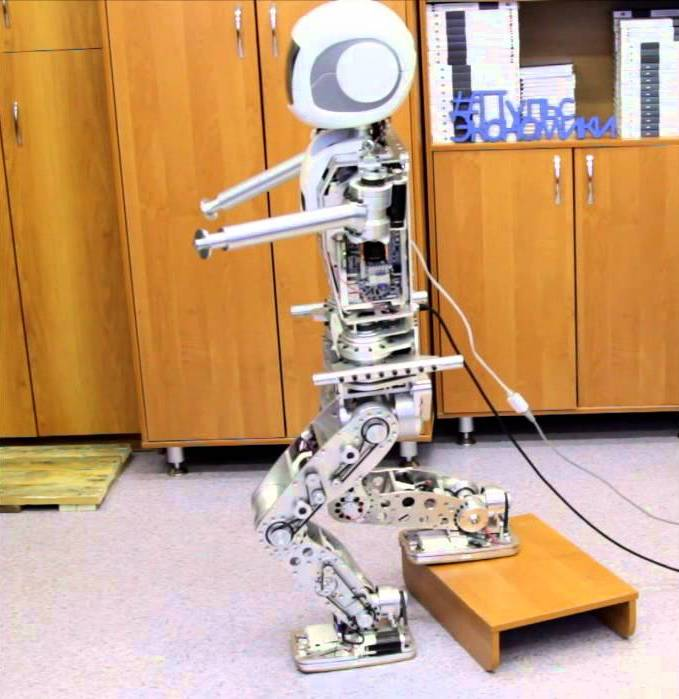
\includegraphics[]{img/ar-600}
	\caption{Антропоморфный робот AR-600E}
	\label{img:ar600}
\end{figure}

Стоит отметить, что именно структура ног отделяет локомоцию тела от движения ног при преодолении препятствий. В результате тело может поддерживать равновесие, что приводит к хорошей адаптации большинства распространенных ландшафтов. Поэтому в последнее время именно шагающие роботы являются наиболее приоритетными в исследованиях, проводимыми в области роботов. Именно ноги являются ключевыми частями конструкции шагающего робота.

Применение шагающих роботов представляет собой довольно обширную область. Это могут быть как гражданские цели, такие как доставка грузов, так и военные и медицинские. Достигнув оптимального подхода с помощью роботизированных механизмов, шагающие роботы смогут выполнять опасные задачи в армии, помогать некоторым людям, использующим инвалидные коляски, приобретать «ходячие» способности. В плане медицины можно получить довольно значительные улучшения, возможно, с протезами, которые работают намного лучше, чем существующие технологии, или даже создание экзоскелетов, которые могли бы позволить человеку с ограниченными двигательными способностями эффективно ходить. В условиях особой опасности, шагающие роботы могут пригодиться военным, полицейским и спасателям. К примеру, можно проводить операции по обнаружению мин и обезвреживанию в суровых условиях с множеством препятствий, где обычные транспортные средства не могут справиться с задачей. Уникальной характеристикой пешеходных транспортных средств является способность двигаться с дискретным размещением ног, что позволяет роботу избегать наступления на мины или другие деликатные объекты.

\section{Инсектоморфные роботы}

Инсектоморфными называется такой вид шагающих роботов, у которых по аналогии с насекомыми (англ. insect - насекомое) располагается три пары конечностей. Фактически, элементарное движение шестиногого шагающего робота может быть достигнуто простым переключением поддержки робота между набором ножек, которые образуют треугольник. Кроме того, для обеспечения статического хождения координация шести ножек может быть осуществлена путем наложения подходящего запаса устойчивости между проекцией грунта центра тяжести робота и многоугольником между опорными лапами.

Другой подход к дизайну шестиногих шагающих роботов можно получить, обратившись к биологическим системам и, таким образом, разработать биологически вдохновленный дизайн робота. Фактически, согласно "техническому замыслу"{}, биологическое вдохновение может быть лишь тривиальным наблюдением того, что некоторые насекомые используют шесть ног, которые полезны для получения устойчивой опоры во время ходьбы, в то время как "биологический замысел"{} означает подражание движению конкретного вида насекомых в каждой детале. В общем, насекомые ходят на нескольких скоростях с различными походками, обладающими свойством статической устойчивости, но одной из ключевых характеристик управления передвижением является распределение.

Таким образом, в отличие от простого управления переключением "технического дизайна"{}, управление распределенной походкой следует рассматривать в соответствии с "биологическим дизайном"{} шестиногого шагающего робота, который пытается эмулировать передвижение конкретного насекомого. Другими словами, вместо централизованной системы управления движением робота можно считать, что различные локальные контроллеры ног обеспечивают управление распределенной походкой.

В ВолгГТУ на кафедре электронных вычислительных машин и систем уже был разработан и собран опытный образец инсектоморфного робота гексопода (рис. \ref{img:hexapod}), реализация управления для которого рассматривается далее в данной работе. Также ведутся работы в области создания более продвинутой модели гексапода, и их оснащение техническим зрением и манипулятором.

\begin{figure}[h!]
	\centering
	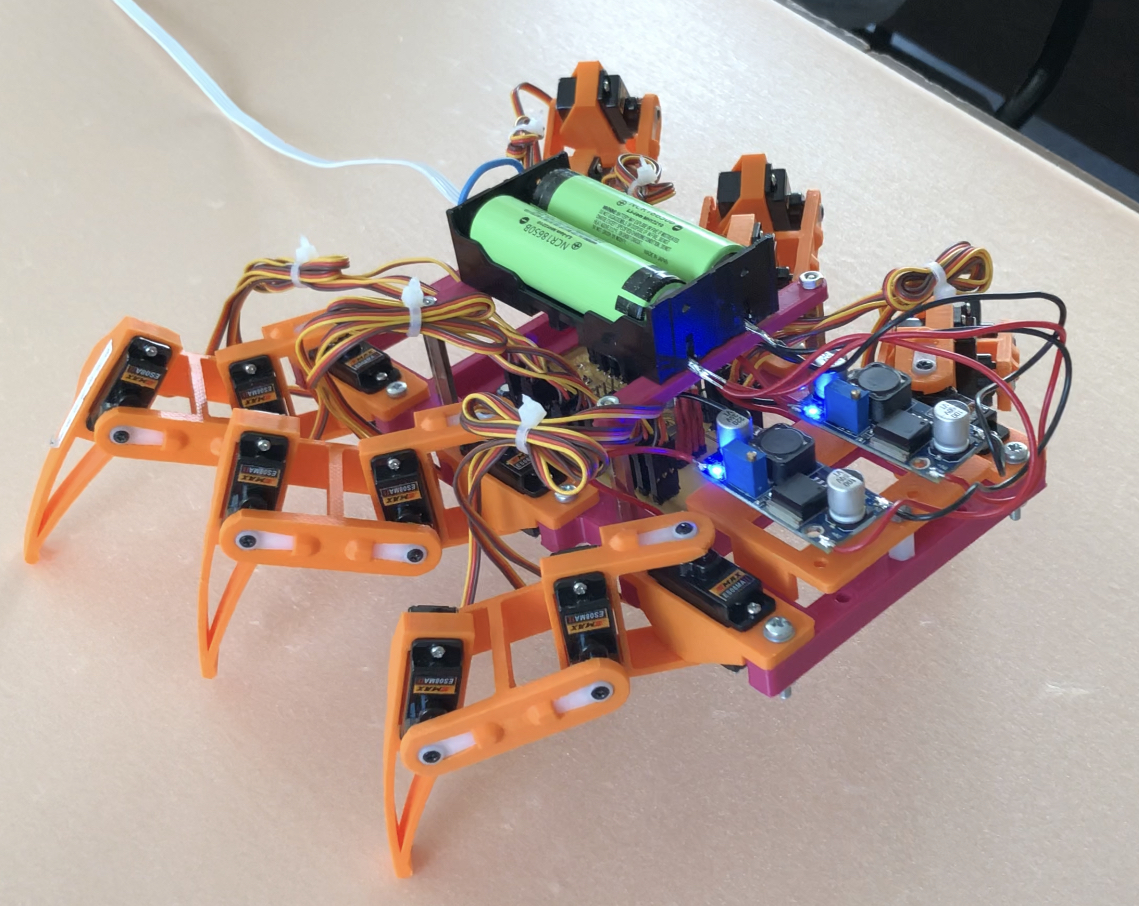
\includegraphics[width=0.65\linewidth]{img/hexapod}
	\caption{Опытная модель гексапода}
	\label{img:hexapod}
\end{figure}

\section{Методы управления роботами}

Решение задачи управления роботами является одной из основополагающих. В общем случае, колесные и гусеничные роботы являются довольно простыми при ручном управлении. Для этого обычно применяются различные пульты дистанционного управления или специальное ПО для компьютера. Простота заключается в том, что как правило, для управления достаточно лишь функции движения прямо, в обратном направлении, а также функций поворота. Все это происходит либо на плоскости, либо в условиях легкого бездорожья. Однако, когда дело касается шагающих роботов все усложняется необходимостью предусмотреть системы обратной связи и алгоритмы для удержания равновесия.

\subsection{Датчики на шагающих роботах}

Датчики обратной связи являются основой динамического баланса и ходьбы в целом. Вот почему уделяется особое внимание выбору подходящих датчиков и их использованию для управления роботом. С другой стороны, существует целый ряд роботов, которые не используют какие-либо датчики на всех и полагаются исключительно на стабильную механическую конструкцию с большой площадью опоры для балансировки и ходьбы.

Рассмотрим датчики, которые применяются в роботах:
\begin{itemize}
	\item Инфракрасные датчики приближения на ногах дают обратную связь о том, соприкасается ли они с землей;
	\item Датчики ускорения в двух осях для измерения динамических сил на роботе, чтобы сбалансировать его;
	\item Пьезо гироскопы используются в качестве альтернативы датчикам ускорения, которые подвержены высокочастотному сервошуму. Поскольку гироскопы только возвращают изменение ускорения, их значения должны быть интегрированы для сохранения общей ориентации;
	\item Инклинометры используются для поддержки гироскопов. Хотя инклинометры нельзя использовать по отдельности из-за их временной задержки, их можно использовать для устранения смещения датчиков и ошибок интеграции гироскопов;
	\item Инфракрасные PSD размещенные в направлениях вперед, влево и вправо, робот может распознавать окружающие препятствия.
	\item Цифровая камера может использоваться двумя способами: либо для поддержки балансировки, либо для обнаружения объектов, пешеходных дорожек и т.д.
\end{itemize}

\subsection{Типы походки и баланс}

Есть два типа походки, используя:

\begin{itemize}
	\item Статический баланс – центр масс робота всегда находится в пределах области поддержки его ноги на земле или объединенной области поддержки его двух ног, если обе ноги находятся на земле.
	\item Динамический баланс - центр тяжести робота может находиться за пределами зоны поддержки его ног во время фазы его походки.
\end{itemize}

Также стоит выделить следующие параметры походки:

\begin{enumerate}
	\item Длина шага;
	\item Высота шага;
	\item Скорость ходьбы;
	\item Угол наклона туловища;
	\item Максимальный угол наклона.
\end{enumerate}

Затем параметры походки обновляются в режиме реального времени в зависимости от датчиков робота. Показания датчика тока сравниваются с требуемыми показаниями датчика в каждый момент времени походки. Различия между текущим и желаемым показаниями датчика приведут к немедлительной адаптации параметров к модели походки.

Модели походки, основанные на статическом равновесии, не очень эффективны. Они требуют больших площадей ног и возможны только относительно медленные походки, чтобы поддерживать динамические силы на низком уровне. Механизмы ходьбы с динамическим балансом, с другой стороны, позволяют создавать роботов с более мелкими ступнями, даже ступнями, которые имеют только одну точку контакта и могут использоваться для гораздо более быстрой ходьбы или даже для бега.

Как было определено ранее, динамическое равновесие означает, что, по крайней мере, на некоторых этапах походки робота его центр масс не поддерживается его ногой. Игнорирование любых динамических сил и моментов означает, что робот упадет, если в реальном времени не будет предпринято противодействие. Существует ряд различных подходов к динамической ходьбе, описанных ниже:

\begin{enumerate}
	\item Нулевой момент это один из стандартных методов динамического баланса и опубликован в ряде статей. Реализация этого метода требует знания всех динамических сил на теле робота, а также всех моментов между ногой и лодыжкой робота. Эти данные можно определить с помощью акселерометров или гироскопов на теле робота, а также датчиков давления в ногах робота или датчиков крутящего момента на лодыжках робота. При всех известных силах контакта и всех динамических силах робота можно рассчитать «точку нулевого момента», которая является динамическим эквивалентом статического центра масс. Если она находится в зоне поддержки ноги робота (или обеих ног) на земле, то робот находится в динамическом равновесии. В противном случае необходимо предпринять корректирующие действия, изменив положение тела робота, чтобы избежать его падения;
	\item Перевернутый маятник - шагающего робота можно смоделировать как перевернутый маятник. Динамического равновесия можно достичь, постоянно отслеживая ускорение робота и адаптируя соответствующие движения ног;
	\item Нейронные сети могут быть использованы для достижения динамического баланса. Конечно, этот подход все еще требует обратной связи с датчиками, как и в других подходах;
	\item Генетические алгоритмы. Популяция виртуальных роботов создается с изначально случайными настройками управления. Роботы с наилучшими характеристиками воспроизводятся с использованием генетических алгоритмов для следующего поколения.

	Такой подход на практике требует наличия системы симуляции механики для оценки производительности каждого отдельного робота, и даже в этом случае для достижения хороших характеристик ходьбы требуется несколько дней использования процессора. Основной проблемой здесь является возможность передачи результатов моделирования обратно физическому роботу;
	\item PID регулятор используется для управления наклоном робота, аналогично случаю статического баланса. Однако нет необходимости заставлять робота стоять прямо. Вместо этого на этапе обучения записывается желаемый передний и боковой наклон тела робота на всех этапах его походки. Позже, при контролировании походки, необходимо добиться этого смещения переднего и бокового наклона с помощью PID регулятора. Для достижения такого наклона можно устанавливать следующие параметры:
	\begin{itemize}
		\item Длина шага;
		\item Высота шага;
		\item Скорость ходьбы;
		\item Наклон торса вперед;
		\item Максимальный боковой сдвиг.
	\end{itemize}
	
	\item Искусственный горизонт. В этом подходе используются не кинетические датчики других подходов, а монокулярная камера в градациях серого. В простой версии черная линия на белом фоне помещается в поле зрения робота. Затем мы можем измерить ориентацию робота путем изменения положения и ориентации линии на изображении. Например, линия будет двигаться к вершине, если робот падает вперед, она будет наклонена под углом, если робот наклоняется влево, и т.д. С более мощным контроллером для обработки изображений, тот же принцип может быть применен даже без необходимости искусственного горизонта. Пока на заднем плане достаточно текстуры, для определения движения робота можно использовать общий оптический поток.
\end{enumerate}

\section{Методы управления инсектоморфными роботами}

Как уже писалось ранее, шестиногий робот в его правильном варианте исполнения должен быть биологически вдохновленным. Эмуляция локомоций палочниковых насекомых должна выполняться посредством прямой ходьбы на разных скоростях и ходьбы по кривым или в разных направлениях. Поэтому стоит рассмотреть некоторые технические аспекты ходьбы для построения математической модели.

\subsection{Координация ног}

Основываясь на рисунке \ref{img:leg_cord}, система отсчета $G'({x'}_G\;{y'}_G\;{z'}_G)$ имеющая начало в $G'$, совпадающая с проекцией на землю центра масс $G$ тела шестиножки и шести систем отсчета $O_{Si}(x_{Si}\;y_{Si}\;z_{Si})$ для $i=1,...,6$, была выбрана для анализа и оптимизации движения каждого конца ноги с целью обеспечения подходящей статической устойчивости при ходьбе.

Таким образом, вкратце, движение каждого конца ноги можно выразить как функцию параметров $^{Si}p_{ix}$ и $_{Si}$, где $^{Si}p_{ix}$ дает положение конца ноги в $O_{Si}(x_{Si}\;y_{Si}\;z_{Si})$ вдоль оси $x$ для фазы опоры, а $_{Si}\in\{0;1\}$  указывает состояние каждого конца ноги, т.е. $_{Si} = 0$ используется для фазы переноса, а $_{Si} = 1$ для фазы опоры, которые выполняются в диапазоне $[PEP_i,AEP_i]$, где $PEP_i$ – это заднее крайнее положение, а $AEP_i$ – переднее крайнее положение каждой конечности. В частности, $L$ – это номинальное расстояние между $PEP0$ и $AEP0$. Траектория каждого конца ноги во время фазы переноса определяется с учетом времени начала и окончания фазы опоры.

\begin{figure}[h!]
	\centering
	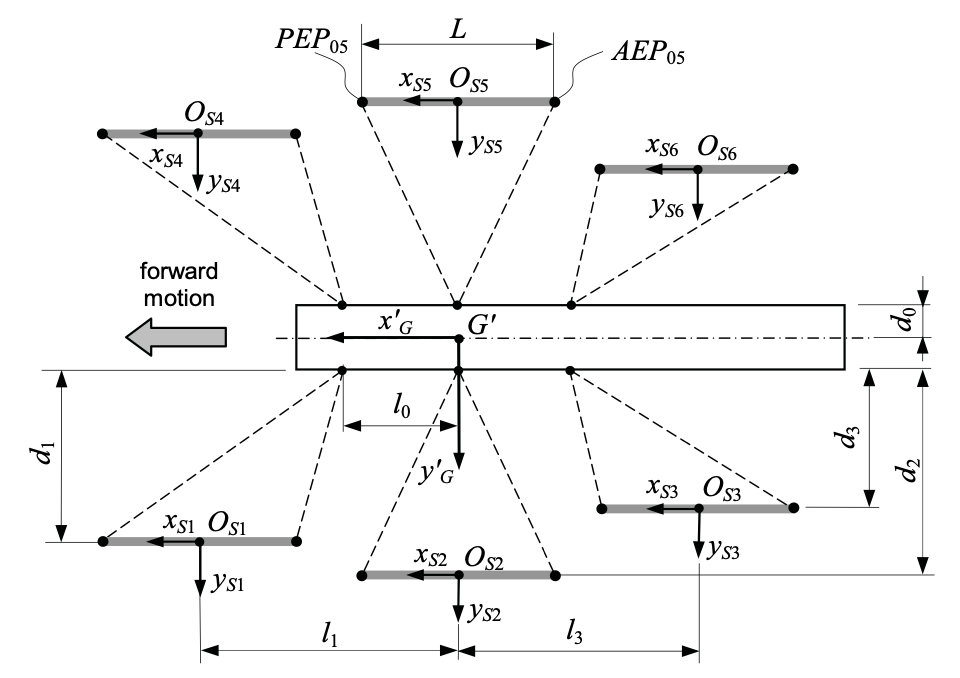
\includegraphics[]{img/leg_cord}
	\caption{Общая схема гексапода}
	\label{img:leg_cord}
\end{figure}

\subsection{Механизм ног}

Кинематическая цепочка с тремя оборотами для каждой ноги используется в целях имитирования структуры ноги палочника, а именно coxa, femur и tibia как показано на рисунке \ref{img:leg_mech}. Непосредственный кинематический анализ каждого механизма ноги формируется между подвижной системой координат $O_{Ti}(x_{Ti}\;y_{Ti}\;z_{Ti})$ тела tibia и системой координат $O_{0i}(x_{0i}\;y_{0i}\;z_{0i})$, которая рассматривается как неподвижная рама, прежде чем она будет соединена с корпусом робота, чтобы сформулировать общую модель гексапода, показанного на рисунке \ref{img:hexapod_model}.

В частности общая матрица преобразования $\mathbf{M}^{0i}_{Ti}$ между подвижной системой координат $O_{Ti}(x_{Ti}\;y_{Ti}\;z_{Ti})$ и неподвижной системой координат определяется как:
\begin{equation}
	\mathbf{M}^{0i}_{Ti}(\vartheta_{1i},\vartheta_{2i},\vartheta_{3i}) =
	\begin{bmatrix}
		r_{11} & r_{12} & r_{13} & ^{0i}p_{ix}\\
		r_{21} & r_{22} & r_{23} & ^{0i}p_{iy}\\
		r_{31} & r_{32} & r_{33} & ^{0i}p_{iz}\\
		0	&	0	&	0	&	1
	\end{bmatrix}  
\end{equation}

Эта матрица получается как произведение между четырьмя матрицами преобразования, которые связывают подвижную систему tibia с тремя типичными опорными звеньями на поворотных суставах (jounts) механизма ноги.

Таким образом, каждая запись $r_{jk}$ в $\mathbf{M}^{0i}_{Ti}$ для $j,k = 1,2,3$ и декартовой компоненты положения вектор $\mathbf{p}_i$ в системе координат $O_{0i}(x_{0i}\;y_{0i}\;z_{0i})$ задается выражением:

\begin{equation}
\begin{array}{l}
	r_{11}=\mathrm{c} \alpha_{0} \mathrm{s} \vartheta_{1 i} ; \quad r_{21}=-\mathrm{c} \vartheta_{1 i} ; \quad r_{31}=-\mathrm{s} \vartheta_{1 i} \mathrm{s} \alpha_{0} \\
	r_{12}=\mathbf{s} \vartheta_{3 i}\left(\mathbf{s} \alpha_{0} \mathbf{s} \vartheta_{2 i}-\mathbf{c} \alpha_{0} \mathbf{c} \vartheta_{1 i} \mathbf{c} \vartheta_{2 i}\right)-\mathbf{c} \vartheta_{3 i}\left(\mathbf{c} \alpha_{0} \mathbf{c} \vartheta_{1 i} \mathbf{s} \vartheta_{2 i}+\mathbf{s} \alpha_{0} \mathbf{c} \vartheta_{2 i}\right) \\
	r_{22}=-\mathrm{s} \vartheta_{1 i} \mathrm{c} \vartheta_{2 i} \mathrm{s} \vartheta_{3 i}-\mathrm{s} \vartheta_{1 i} \mathrm{s} \vartheta_{2 i} \mathrm{c} \vartheta_{3 i}\\
	r_{32}=\mathbf{s} \vartheta_{3 i}\left(\mathrm{c} \alpha_{0} \mathrm{s} \vartheta_{2 i}+\mathrm{s} \alpha_{0} \mathrm{c} \vartheta_{1 i} \mathrm{c} \vartheta_{2 i}\right)+\mathrm{c} \vartheta_{3 i}\left(\mathrm{s} \alpha_{0} \mathrm{c} \vartheta_{1 i} \mathrm{s} \vartheta_{2 i}+\mathrm{c} \alpha_{0} \mathrm{c} \vartheta_{2 i}\right)\\
	r_{13}=\mathrm{c} \vartheta_{3 i}\left(\mathrm{c} \alpha_{0} \mathrm{c} \vartheta_{1 i} \mathrm{c} \vartheta_{2 i}-\mathrm{s} \alpha_{0} \mathrm{s} \vartheta_{2 i}\right)-\mathrm{s} \vartheta_{3 i}\left(\mathrm{c} \alpha_{0} \mathrm{c} \vartheta_{1 i} \mathrm{s} \vartheta_{2 i}+\mathrm{s} \alpha_{0} \mathrm{c} \vartheta_{2 i}\right)\\
	r_{23}=\mathrm{s} \vartheta_{1 i} \mathrm{c} \vartheta_{2 i} \mathrm{c} \vartheta_{3 i}-\mathrm{s} \vartheta_{1 i} \mathrm{s} \vartheta_{2 i} \mathrm{s} \vartheta_{3 i}\\
	r_{33}=-\mathrm{c} \vartheta_{3 i}\left(\mathrm{s} \alpha_{0} \mathrm{c} \vartheta_{1 i} \mathrm{c} \vartheta_{2 i}+\mathrm{c} \alpha_{0} \mathrm{s} \vartheta_{2 i}\right)+\mathrm{s} \vartheta_{3 i}\left(\mathrm{s} \alpha_{0} \mathrm{c} \vartheta_{1 i} \mathrm{s} \vartheta_{2 i}-\mathrm{c} \alpha_{0} \mathrm{c} \vartheta_{2 i}\right)\\
	\begin{aligned}
		^{0 i} p_{i x} &=\left[\mathrm{c} \vartheta_{3 i}^{2}\left(\mathrm{c} \alpha_{0} \mathrm{c} \vartheta_{1 i}^{2} \mathrm{c} \vartheta_{2 i}-\mathrm{s} \alpha_{0} \mathrm{s} \vartheta_{2 i}\right)-\mathrm{s} \vartheta_{3 i}\left(\mathrm{c} \alpha_{0} \mathrm{c} \vartheta_{1 i} \mathrm{s} \vartheta_{2 i}+\mathrm{s} \alpha_{0} \mathrm{c} \vartheta_{2 i}\right)\right] a_{3}+\\
		&+\left(\mathrm{c} \alpha_{0} \mathrm{c} \vartheta_{1 i} \mathrm{c} \vartheta_{2 i}-\mathrm{s} \alpha_{0} \mathrm{s} \vartheta_{2 i}\right) a_{2}+\mathrm{c} \alpha_{0} \mathrm{c} \vartheta_{1 i} a_{1}
	\end{aligned}\\
	^{0 i} p_{i y}=a_{3}\left(\mathrm{s} \vartheta_{1 i} \mathrm{c} \vartheta_{2 i} \mathrm{c} \vartheta_{3 i}-\mathrm{s} \vartheta_{1 i} \mathrm{s} \vartheta_{2 i} \mathrm{s} \vartheta_{3 i}\right)+\left(\mathrm{s} \vartheta_{1 i} \mathrm{c} \vartheta_{2 i}\right) a_{2}+\mathrm{s} \vartheta_{1 i} a_{1}\\
	\begin{aligned}
		^{0 i} p_{i z} &=\left[-c \vartheta_{3 i}\left(\mathrm{s} \alpha_{0} \mathrm{c} \vartheta_{1 i} \mathrm{c} \vartheta_{2 i}+\mathrm{c} \alpha_{0} \mathrm{s} \vartheta_{2 i}\right)+\mathrm{s} \vartheta_{3 i}\left(\mathrm{s} \alpha_{0} \mathrm{c} \vartheta_{1 i} \mathrm{s} \vartheta_{2 i}-\mathrm{c} \alpha_{0} \mathrm{c} \vartheta_{2 i}\right)\right] a_{3}+\\
		&-\left(\mathrm{s} \alpha_{0} \mathrm{c} \vartheta_{1 i} \mathrm{c} \vartheta_{2 i}-\mathrm{c} \alpha_{0} \mathrm{s} \vartheta_{2 i}\right) a_{2}-\mathrm{s} \alpha_{0} \mathrm{c} \vartheta_{1 i} a_{1},
	\end{aligned}
\end{array}
\end{equation}

где $\vartheta_{1i},\;\vartheta_{2i}$ и $\vartheta_{3i}$ переменные углов суставов  каждой из ножек $(i=1,...,6)$, $\alpha_0$ – угол первой оси соединения с осью $z_{0i}$, а $a_1, a_2, a_3$ – длины coxa, femur и tibia соответственно. 

Обратный кинематический анализ механизма ног формируется при помощи алгебраического похода. Таким образом, когда декартовы компоненты вектора положения $\mathbf{p}_i$ заданы в системе координат $O_{Fi}(x_{Fi}\;y_{Fi}\;z_{Fi})$ переменные углы соединения $\vartheta_{1i}, \vartheta_{2i}, \vartheta_{3i} (i=1,...,6)$ можно выразить как:

\begin{equation}
	\vartheta_{1i}=atan2(^{Fi}p_{iy}, ^{Fi}p_{ix}) 
\end{equation}

и

\begin{equation}
	\vartheta_{3i}=atan2(s\vartheta_{3i}, c\vartheta_{3i}) 
\end{equation}

где

\begin{equation}
\begin{array}{l}
	\mathrm{c} \vartheta_{3 i}=\frac{\left(^{F i} p_{i x}\right)^{2}+\left(^{F i} p_{i y}\right)^{2}+\left(^{F i} p_{i z}\right)^{2}+a_{1}^{2}-2 a_{1} \sqrt{\left(^{F i} p_{i x}\right)^{2}+\left(^{F i} p_{i y}\right)^{2}}-a_{2}^{2}-a_{3}^{2}}{2 a_{2} a_{3}},\\
	\mathbf{s} \vartheta_{3 i}=\pm \sqrt{1-\mathrm{c}^{2} \vartheta_{3 i}}
\end{array}
\end{equation}

\begin{figure}[h!]
	\centering
	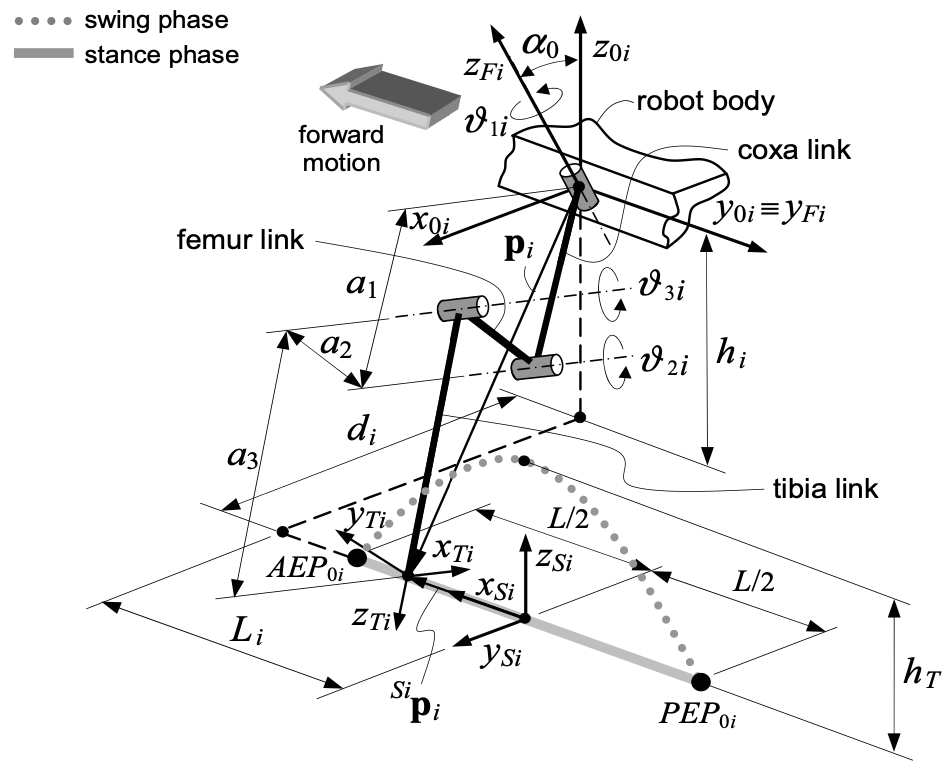
\includegraphics[]{img/leg_mech}
	\caption{Механизм 3R ноги шестиногого шагающего робота}
	\label{img:leg_mech}
\end{figure}

И в свою очередь:
\begin{equation}
	v_{2i}=atan2(s\vartheta_{2i}, c\vartheta_{2i}),
\end{equation}
где
\begin{equation}
\begin{array}{l}
\mathrm{s} \vartheta_{2 i}=-\frac{a_{3} \mathrm{s} \vartheta_{3 i}(\sqrt{\left(^{F i} p_{i x}\right)^{2}+\left(^{F i} p_{i y}\right)^{2}})+^{F i} p_{i z}\left(a_{2}+a_{3} \mathrm{c} \vartheta_{3 i}^{2}\right)}{a_{2}^{2}+a_{3}^{2}+2 a_{2} a_{3} \mathrm{c} \vartheta_{3 i}} \\
\mathrm{c} \vartheta_{2 i}=-\frac{^{F i}p_{i z}+\mathrm{s} \vartheta_{2 i}\left(a_{2}+a_{3} \mathrm{c} \vartheta_{3 i}\right)}{a_{3} \mathrm{s} \vartheta_{3 i}}
\end{array}.
\end{equation}
Таким образом, уравнения (1-7) позволяют сформулировать общую кинематическую модель шестиногого робота, что описывается ниже.

\subsection{Кинематическая модель шестиного шагающего робота}

Полагаясь на рисунок \ref{img:leg_mech} и \ref{img:hexapod_model}, кинематическая модель шестиногого шагающего робота сформулирована посредством прямого кинематического анализа между движемой системой координат $O_{Ti}(x_{Ti}\;y_{Ti}\;z_ {Ti})$ звена tibia и инерционной системой координат $O(X\;Y\;Z)$. 

В общем, шестиногий шагающий робот имеет 24 степени свободы, где 18 степеней свободы задаются значениями $\vartheta_{1i},\vartheta_{2i},\vartheta_{3i}(i=1,...,6)$ для шести механизмов ног 3R, а 6 степеней свободы определяются как тело робота, которые уменьшаются в этом случае только на 1 градус – это дано $X_G$, чтобы рассмотреть чистый переход тела робота вдоль оси $X$.

Таким образом, уравнение движения $X_G(t)$ тела робота назначается в качестве входных данных для предложенного алгоритма, в то время как $\vartheta_{1i}(t), \vartheta_{2i}(t), \vartheta_{3i}(t)$ для $i=1,...,6$ выражены посредством обратного кинематического анализа шести механизмов ног 3R, когда дано уравнение движения каждого конца ноги и задана их форма траектории во время фазы переноса.

В частности, матрица преобразования $\mathbf{M}_G$ системы координат $G(x_G\;y_G\;z_G)$ на корпусе робота относительно инерционной системы координат $O(X\;Y\;Z)$ выражается как:

\begin{equation}
	\mathbf{M}_G(X_G) =
	\begin{bmatrix}
		1 & 0 & 0 & p_{Gx}\\
		0 & 1 & 0 & p_{Gy}\\
		0 & 0 & 1 & p_{Gz}\\
		0 &	0 &	0 &	1
	\end{bmatrix}
	,  
\end{equation}
где $p_{GX}=X_G, \; p_{GY}=0$ и $p_{GZ} = h_G$.

Матрица преобразования $\mathbf{M}^G_{Bi}$ системы координат $O_{Bi}(x_{Bi}\;y_{Bi}\;z_{Bi})$ на корпусе робота относительно системы координат $G(x_G\;y_G\;z_G)$ выражается как:

\begin{equation}
	\mathbf{M}^G_{Bi} = 
	\begin{cases}
		\begin{bmatrix}
			0 	& 1	& 0 & 	d_0	\\
			-1 	& 0 & 0 & 	l_i	\\
			0 	& 0 & 1 & 	0	\\
			0 	& 0 & 0 &	1
		\end{bmatrix}
		,i = 1,2,3\\
				\begin{bmatrix}
			0 	& -1 	& 0 & 	d_0	\\
			1 	& 0     & 0 & 	-l_i	\\
			0 	& 0 		& 1 & 	0	\\
			0 	& 0 		& 0 &	1
		\end{bmatrix}
		,i = 4,5,6\\
	\end{cases}
	,
\end{equation}
где $l_1 = l_4 = -l_0, l_2 = l_5=0, l_3=l_6=l_0$.

Поэтому прямая кинематическая функция шагающего робота определяется как:

\begin{equation}
\mathbf{M}_{T i}\left(X_{G}, \vartheta_{1 i}, \vartheta_{2 i}, \vartheta_{3 i}\right)=\mathbf{M}_{G}\left(X_{G}\right) \mathbf{M}_{B i}^{G} \mathbf{M}_{0 i}^{B i} \mathbf{M}_{T i}^{0 i}\left(\vartheta_{1 i}, \vartheta_{2 i}, \vartheta_{3 i}\right)
,
\end{equation}
где $\mathbf{M}^{Bi}_{0i} = \mathbf{I}$, является $\mathbf{I}$ единичной матрицей. Углы суставов (joints) механизмов ног получены за помощью обратного кинематического анализа. Кроме того матрица преобразования $\mathbf{M}^{Bi}_{Si}$ имеет вид:

\begin{equation}
	\mathbf{M}^{Bi}_{Bi} = 
	\begin{cases}
		\begin{bmatrix}
			0 	& -1	 & 0 & 	L_i	\\
			1 	& 0  & 0 & 	d_i	\\
			0 	& 0  & 1 & 	-h_i	\\
			0 	& 0  & 0 &	1
		\end{bmatrix}
		,i = 1,2,3 \\
				\begin{bmatrix}
			0 	& 1 	& 0 & 	L_{i-3}	\\
			-1 	& 0 & 0 & 	-d_{i-3}\\
			0 	& 0 & 1 & 	-h_i	\\
			0 	& 0 	& 0 &	1
		\end{bmatrix}
		,i = 4,5,6\\
	\end{cases}
	,
\end{equation}
где $L_1 = l_1 - l_0, L_2=0$ и $L_3=l_3-l_0$ c $L_i$, показанной на рисунке \ref{img:leg_mech}. Наконец, положение каждого конца ноги в системе координат $O_{Fi}(x_{Fi}\;y_{Fi}\;z_{Fi})$

\begin{equation}
^{F i} \mathbf{p}_{i}(t)=\mathbf{M}_{0 i}^{F i} \mathbf{M}_{B i}^{0 i} \mathbf{M}_{S i}^{B i} \;^{Si}\mathbf{p}_{i}(t),
\end{equation}

где зная матрицу $\mathbf{M}_{S i}^{B i}$ легко можно получить, зная угол $\alpha_0$.

Cледовательно, подставляя декартовы компоненты $^{Fi}\mathbf{p}_i(t)$ в уравнения(3),(5) и (7) могут быть получены углы суставов $\vartheta_{1i},\vartheta_{2i},\vartheta_{3i}(i=1,...,6)$.

\begin{figure}[h!]
	\centering
	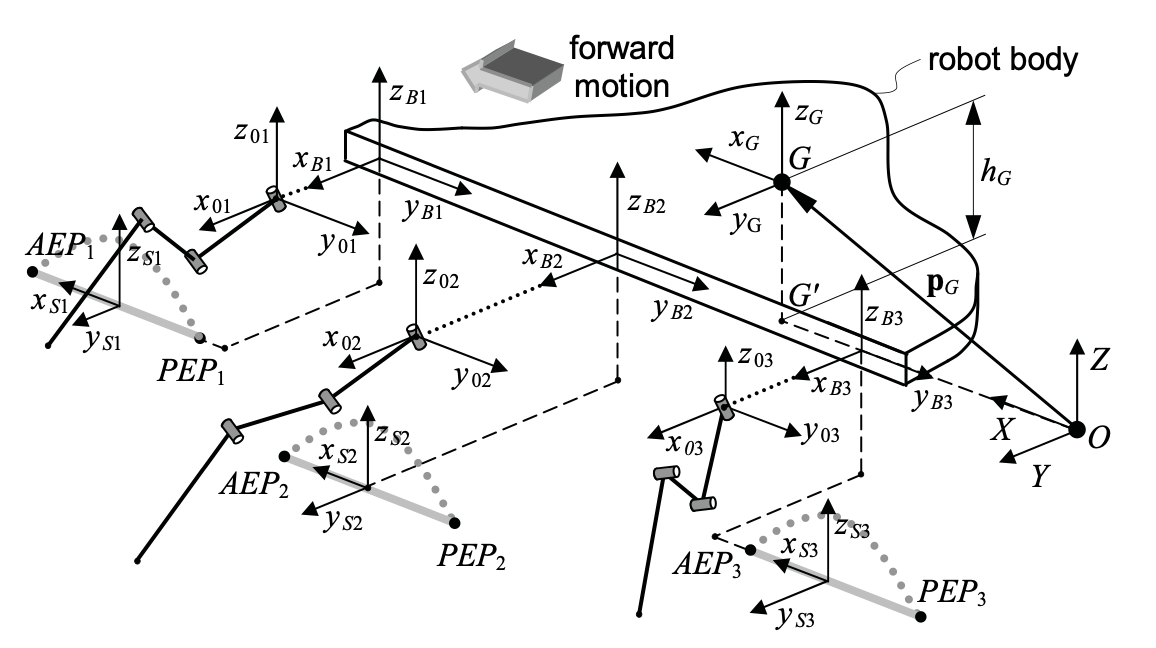
\includegraphics[width = \linewidth]{img/kinematic_scheme}
	\caption{Кинематическая схема шестиногого шагающего робота}
	\label{img:hexapod_model}
\end{figure}

\subsection{Выводы по главе}

Был проведен обзор шагающих роботов, а также инсектоморфных, как подвида. Рассмотрены главные достоинства шагающих роботов перед колесными и гусеничными роботами. Приведен подробный анализ существующих методов управления шагающими роботами, а также разбор кинематической модели инсектоморфного робота, построенного по аналогии с насекомым палочником.